\section{Variations}
\label{sec:variations}
Many variations of the basic MCTS approach have been proposed in research. This section presents some notable developments in recent years.
\subsection{Real-Time}
In the context of developing agents to play the arcade game Ms Pac-Man \cite{pepels2014real} propose a variety of modifications to MCTS that enable real-time search, i.e., search within invariable time constraints. To this end they define an array of modifications that are specific to the game in their formulation but can be generalized. Two of them are described below.


\begin{figure}[htbp]
    \centering
    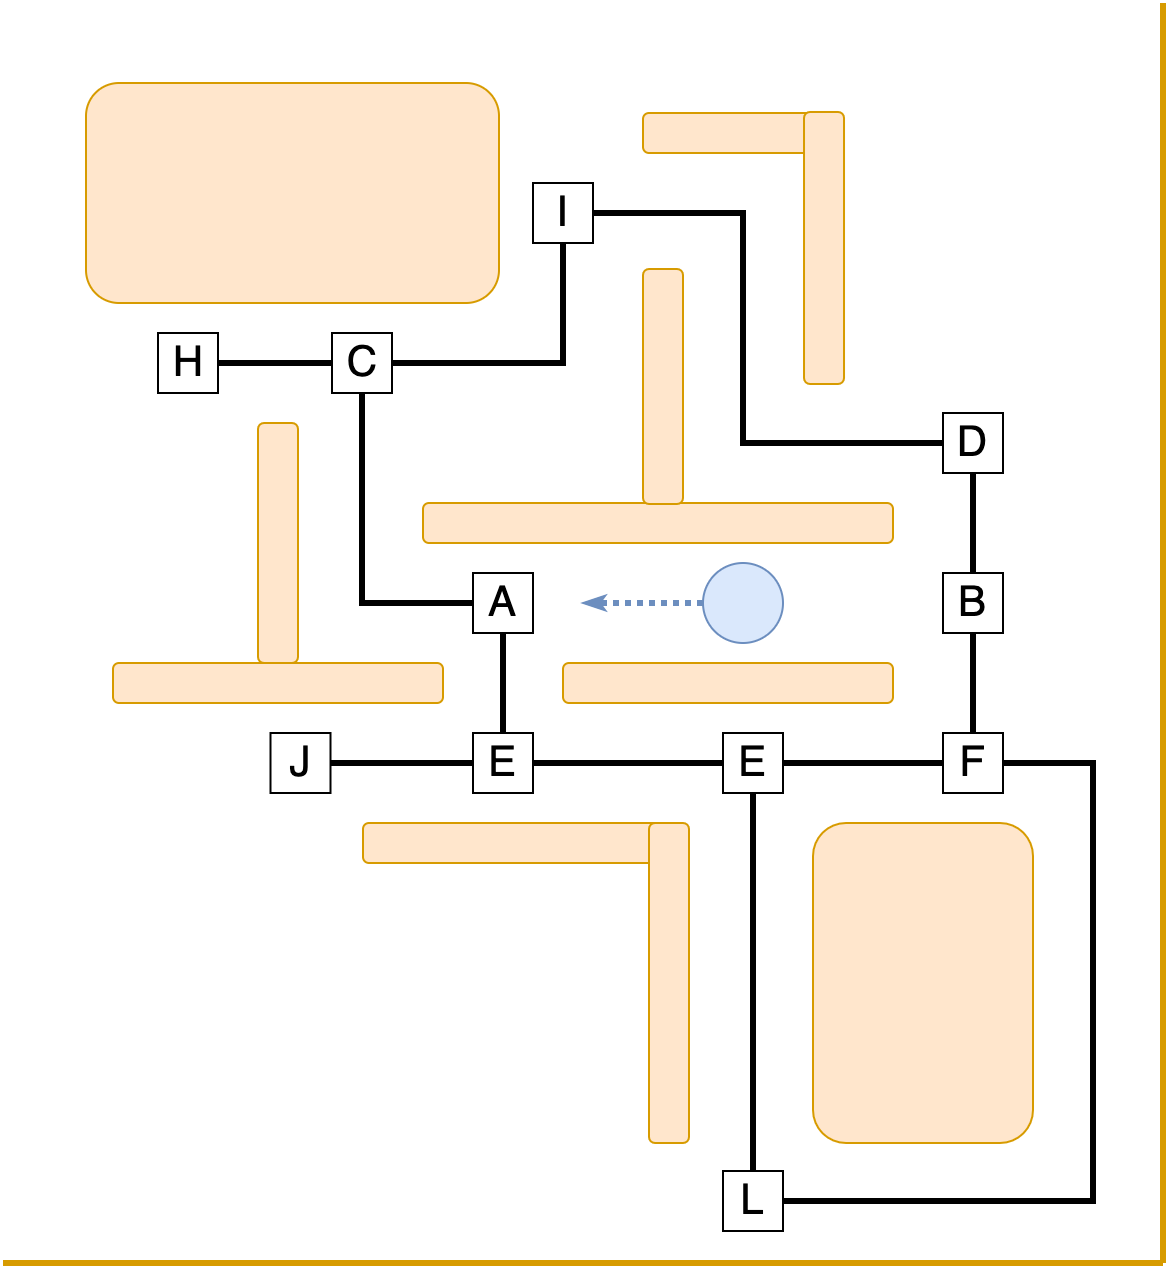
\includegraphics[width=0.5\textwidth]{img/mspacman.png}\\
    \vspace*{0.7cm}
    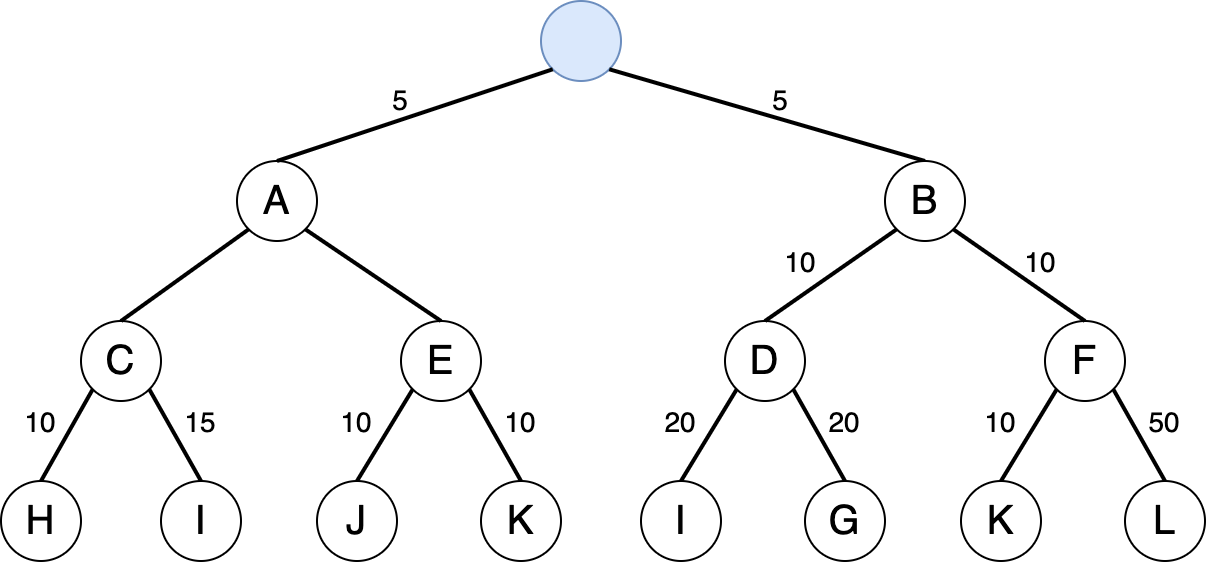
\includegraphics[width=0.6\textwidth]{img/mspacman-tree.png}
    \caption{A sample game state of Ms. Pac-Man and its corresponding search tree.}
    \label{fig:mspacman}
\end{figure}
One aspect concerns the creation and use of the search tree. This tree discretizes the complex game state. As shown in figure. Nodes represent junctions in the game maze. These nodes are connected by edges with an associated length representing the distance that the player has to travel to reach them. Within \enquote{corridors} there are no decisions to be made and moves that lead back to the parent are not considered and modelled. Thirdly, opponents are not represented as nodes at all. Their movements are simulated while the player traverses the tree and are an additional factor in the game state given by the player's nodes, making these states themselves only approximations. Upon reaching a node (i.e. a junction) the children considered in the expansion step are those that are \begin{enumerate*}[label=\roman*)]
    \item directly reachable (i.e. neighbors of the current junction)
    \item have a distance that would make the length of the search path no longer than a parameter $T_{path}$.
\end{enumerate*} The last requirement limits the depth of the search tree.

The other aspect is the reuse of the search tree. Since the quality of the results of Monte Carlo methods depends on the number of simulations which is necessarily small in real-time scenarios. Additionally, Pac-Man follows a long-term reasoning heuristic (a \textit{plan}). Starting the search over every turn makes such long term reasoning impossible. However, simply keeping an old plan may lead to bad decisions since the values change over time, making the information used outdated. Two techniques are used to mitigate this problem when reusing trees.

\begin{enumerate}[label=\arabic*)]
    \item \textit{Rule-Based Reuse}: If one of a set of conditions is met the existing tree is discarded and a new one is built. While the exact conditions are game-specific, the death of the player is a prominent example.
    \item \textit{Continuous Decay}: The values stored at nodes describing the state of the game are multiplied by a parameter $\gamma \in [0,1]$ at the beginning of each turn. Setting this parameter to zero means no reuse since all values are discarded and setting it to one means no decay at all.
\end{enumerate}

\cite{soemers2016enhancements} present eight enhancements for real-time MCTS, again in the context of games. Four examples are:
\begin{enumerate}[label=\alph*)]
    \item \textit{Breadth-First Tree Initialization}: Sometimes the number of simulations that can be executed during a turn is smaller than the number of possible actions. This can lead to near-random behavior like selecting an action that leads to a direct loss. This problem is mitigated prior to the start of MCTS by executing a one-step Breadth-First Search from the root node generating all its successors. Then for every successor $M$ simulations are executed and their results backpropagated. Now the actual search is started where there is now information available to avoid bad first moves. One modification is to save the results of the $M$ simulations directly in the successor nodes for reuse later and thereby reduce the overhead.
    \item \textit{Loss Avoidance}: If there are many loss states in a game tree the estimation of a node generated by MCTS can be overly negative. That is, if a node has many children leading to a loss state and only a few leading to a win state simulations will mostly encounter loss nodes and return a low value. \textit{Loss Avoidance} deals with this problem as follows: The first time a node is visited losses are ignored and alternatives are explored immediately. More precisely, any time a simulation involving an unexplored node ends in a loss the result is not backpropagated right away but instead the algorithm backtracks and explores the neighboring nodes. After all alternatives are exhausted only the result of the highest value is backpropagated back to the root.
    \item \textit{Novelty-Based Pruning}: Often there are many redundant paths through the game tree. The aim of \textit{Novelty-Based Pruning} is to prune nodes in such redundant paths. To this end, a novelty measure $nov(s)$ is introduced which assigns each state (node) a score that is high if it is redundant, i.e. similar to other states in its neighborhood $N(s)$. This set consists of the union of four sets of states, namely \begin{enumerate}[label=\roman*)]
        \item the siblings on the \enquote{left} side of $s$
        \item the parent of $s$, denoted as $p(s)$
        \item the siblings of $p(s)$
        \item the neighborhood of $p(s)$, i.e. $N(p(s))$
    \end{enumerate}
    
    Now we can define $nov(s,N(s))$ as the size of the smallest tuple of features that is true in $s$ and not true in $N(s)$. States with a high $nov(\cdot)$ value are pruned and the number of \enquote{unnecessary} paths reduced.
    \item \textit{Knowledge-Based Evaluations}: Depending on the game it is often the case that simulations do not find a terminal state or one that changes the score. In such cases the same value is returned for most nodes and no meaningful information is gained. To distinguish between states that have the same evaluation a heuristic function is used. First any object in the game is assigned a type (say, \enquote{wall}, \enquote{enemy}, \enquote{friendly}) and a weight $w_i > 0$ is computed for every type. Let $\Delta_{s_0}$ and $\Delta_{s_T}$ denote the evaluation of the current game state and that of the final state of a simulation. Let $d_0(i)$ and $d_T(i)$ denote the distance to the closest object of type $i$ from the initial state and the terminal state, computed via the $A^\star$ pathfinding algorithm. Now a heuristic value given by the equation $\sum_i w_i \cdot (d_0(i) - d_T(i))$ is added to $\Delta_{s_T}$. Intuitively this heuristic computes the distance to \enquote{interesting} objects of state $s_T$ compared to $s_0$. 
\end{enumerate}
\subsection{Multiple Agents}
\paragraph{Multi-Agent MCTS}
Most MCTS research is focussed on competitive games, i.e. games where two or more players play against each other and each aim to win themselves. \cite{zerbel2019multiagent} focusses instead on cooperation between multiple agents. That is games where multiple agents still have individual policies but have to coordinate them to achieve a common goal. ... 

\begin{algorithm}[htbp]
\begin{algorithmic}
\For{each \textit{Episode}}
\For{each \textit{Agent}}
\State standard MCTS
\EndFor
\For{each \textit{Agent}}
\State select best policy from tree
\State execute actions in best policy
\EndFor
\For{each \textit{Agent}}
\State evaluate policy
\State update tree
\EndFor
\State reset agents
\EndFor
\end{algorithmic}
\caption{Multi-Agent MCTS.}
\label{alg:mamcts}
\end{algorithm}
\todo{content, episode, MAG, actions?}
\paragraph{Decentralized, Multi-Agent Planning}
In the context of robot move planning \cite{best2019dec} proposes a variation of MCTS that is both decentralized and online called \textit{Dec-MCTS}. Each robot is part of a joint action space, it optimizes its own planning locally via a probabilistic distribution over all plans and periodically exchanges its search tree with other robots in a compressed version. This information is then used to update its own plans (i.e., the distribution thereof). To this end, they also define a new tree expansion policy called \textit{D-UCT} which is, in turn, a generalization of \textit{D-UCB} \cite{garivier2011upper}.

The problem to be solved can be stated as follows: Each robot $r$ in the set of robots $\{1,\ldots,R\}$ plans its personal sequence of future actions $ \mathbf{x}^r \coloneqq (x_1^r,x_2^r,\ldots)$. An action $x_j^r$ has a cost $c_j^r$ and the cost of all actions must not exceed the robots budget $B^r$.
%formally: It must hold that $\sum_{x_j^r \in \mathbf{x}^r} c_j^r \leq B^r$. 
Let $\mathcal{X}^r$ denote the set of all possible action sequences $\mathbf{x}^r$ for a robot r and let $\mathbf{x} \coloneqq \{\mathbf{x}
^1, \ldots , \mathbf{x}^R\}$ denote this set for all robots. 
%Further let $\mathbf{x}^{(r)}$ denote the set of all possible sequences for all robots except $r$, consequentially $X^{(r)}$ is the set of all possible $\mathbf{x}^{(r)}$  
Now the aim is to maximize a global objective function $g(\mathbf{x})$. This function is known to each robot but not the action sequences selected by the others. This information must be exchanged in an asynchronous manner which usually is additionally restricted in other ways (e.g. limits on size, number and timing of messages). 
The proposed Algorithm Dec-MCTS is displayed in Figure \ref{fig:dec_mcts}. It consists of three phases and is running asynchronously on all robots until the computational budget is exhausted. In particular the algorithm is fault tolerant with respect to the success of the communication with other robots. Consider robot $r$ running the $n$-th iteration of the algorithm. Its current plan is defined as a probability distribution $q^r_n$ over all action sequences $\mathcal{X}^r$. To make the problem tractable the actual domain $\Hat{\mathcal{X}}^r_n \subset \mathcal{X}^r$ ... refined (i.e., the probability is zero for all action sequences not in $\Hat{\mathcal{X}}^r_n$)

Focus on step one. The search tree $\mathcal{T}^r$ contains only the actions of robot $r$, each edge representing one action and paths representing valid action sequences. Both the tree and default policies of the standard MCTS-algorithm are adapted. To define the tree policy a discounted version of UCT is used. ...
Parameter $\gamma \in [0,1]$ ...
\begin{equation*}
    N_\gamma(s) \coloneqq \sum_{u = 1}^t \gamma^{t-u} \cdot \mathbb{I}_t(s)
\end{equation*}
The function $\mathbb{I}_t(s)$ is equal to one if $s$ has been selected at epoch $t$ and zero otherwise.
\begin{equation*}
    \Bar{Q}_\gamma(s) \coloneqq \frac{1}{N_\gamma(s)}\sum_{u = 1}^t  \gamma^{t-u} \cdot Q^u(s) \cdot \mathbb{I}_u(s)
\end{equation*}
Now the child selection function is given via:
\begin{equation*}
    \text{D-UCT}(\gamma,s) =  \Bar{Q}_\gamma(s) + C_p \cdot \sqrt{\frac{2 \ln N_\gamma(s)}{N_\gamma(s')}}
\end{equation*}

\begin{figure}
    \centering
    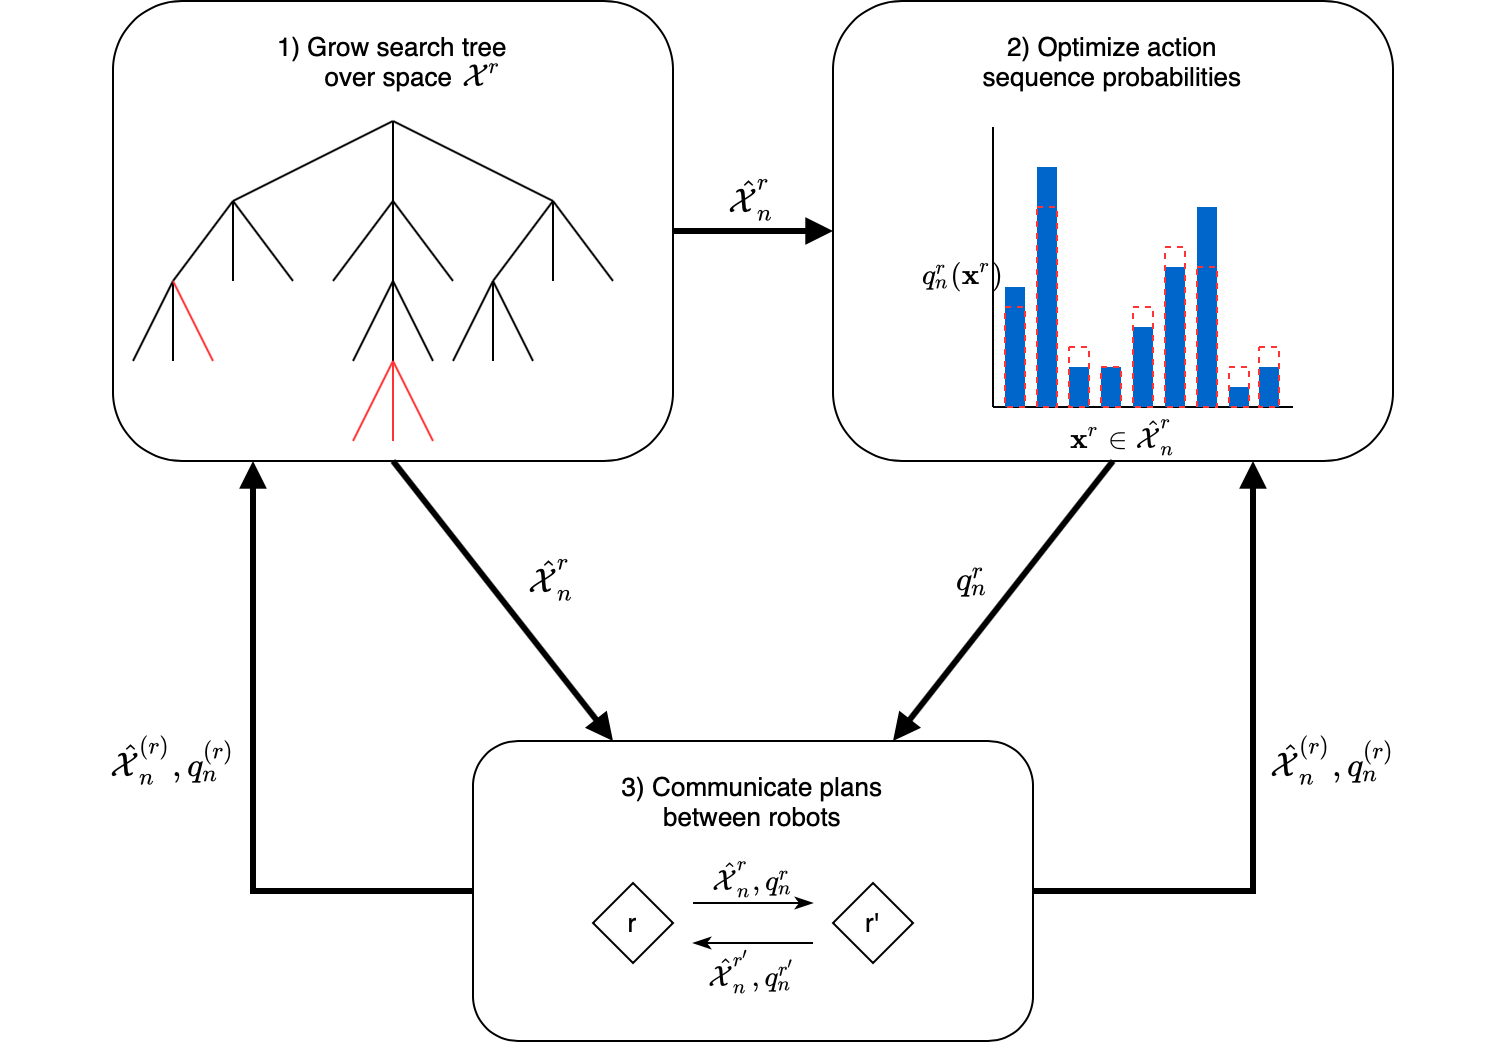
\includegraphics[width=0.9\textwidth]{img/dec-mcts.png}
    \caption{The three basic steps of Dec-MCTS.}
    \label{fig:dec_mcts}
\end{figure}
\subsection{Heuristics}
\label{ss:heuristics}
\paragraph{AMAF and RAVE} There exist many heuristics for MCTS. That is use-case specific enhancements and modifications of the basic MCTS steps (most importantly tree and default policy). In the context of MAB and UCT child selection one important heuristic is \textit{All Moves As First} (\textit{AMAF}) \cite{gelly2007combining} and its enhancement \textit{Rapid Action Value Estimation} (\textit{RAVE}) \cite{gelly2011monte}. AMAF treats every action used during the simulation (i.e. chosen by the default policy) as if it was chosen by the tree policy. This is illustrated in Figure \ref{fig:amaf} in the context of Tic-Tac-Toe. Beginning from the given state UCT selects $(C,2)$ as the next black position and $(A,1)$ for the next white one. Then the progress of the game is simulated with $(B,1)$ black, $(A,3)$ white and $(C,3)$ black, leading to the terminal state displayed and resulting in a win for black. During the backpropagation the values for the nodes visited by UCT are updated as before. But due to AMAF more nodes are updated: Since $(B,1)$ (as well as the others) could have been chosen by UCT and was used during the simulation its statistics are updated as well. The value generated this way is called \textit{AMAF score} and is generally separate from the UCT value.
\begin{figure}
    \centering
    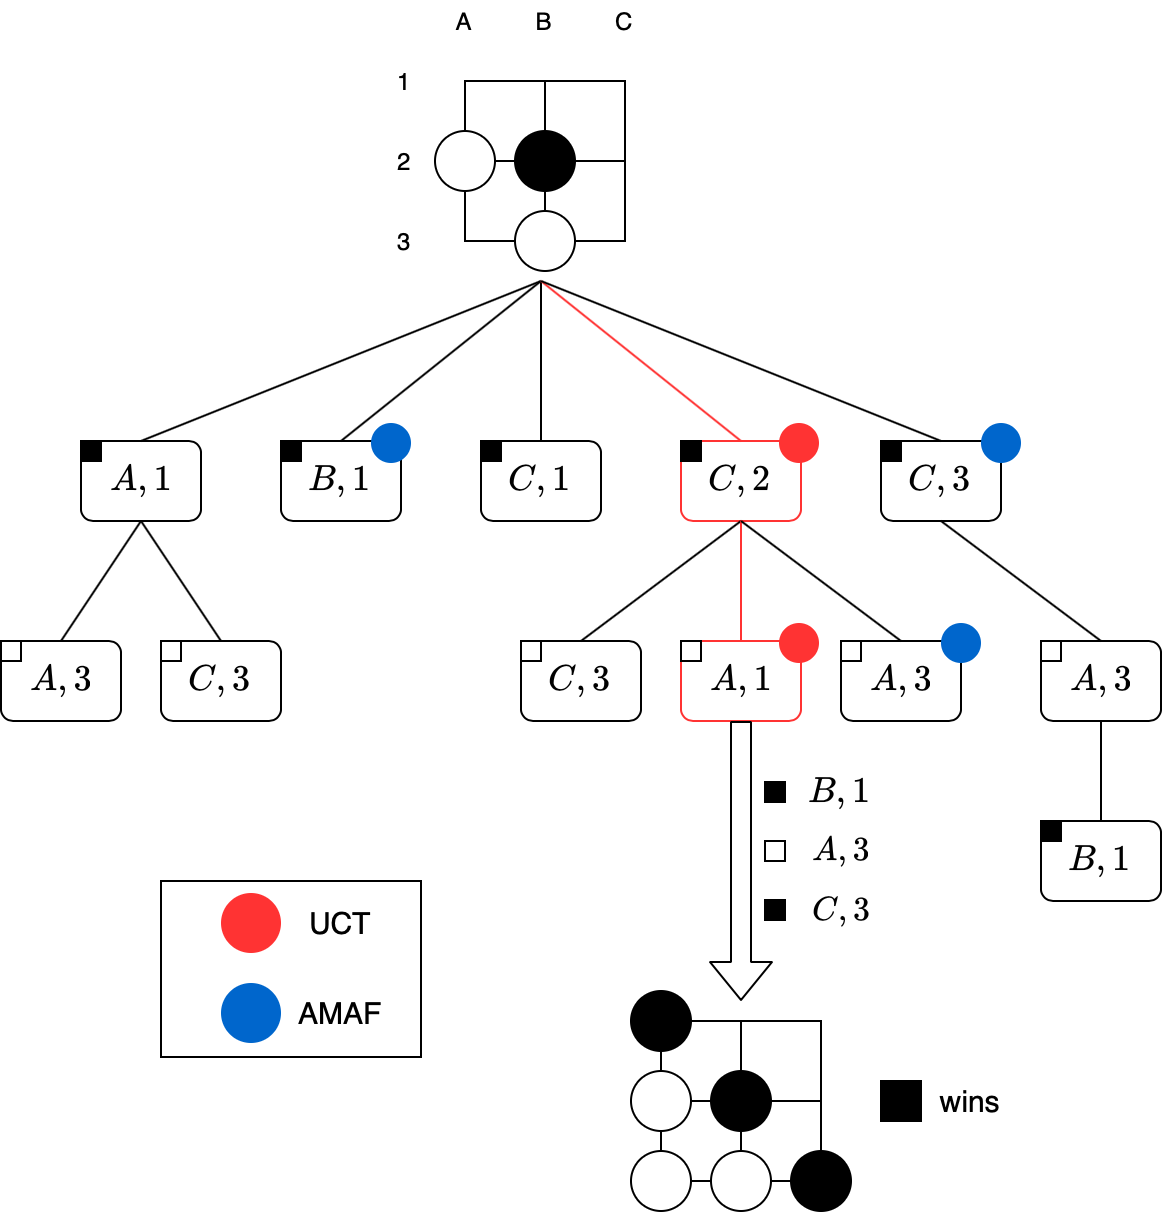
\includegraphics[width=0.7\textwidth]{img/amaf.png}
    \caption{The AMAF-heuristic updates all nodes that are used in the simulation as if they were selected by UCT directly.}
    \label{fig:amaf}
\end{figure}
\textit{RAVE} is a way of combining the UCT value $Q(\cdot)$ and AMAF score $AMAF(\cdot)$ for an action $a$ at a state $s$ via the equation:
\begin{equation}
    \beta(s) \cdot Q(s,a) + (1 - \beta(s)) \cdot AMAF(s',a)
    \label{eq:rave}
\end{equation}
where 
\begin{equation*}
    \beta(s) = \sqrt{\frac{K}{3 \cdot N(s) + K}}
\end{equation*}
$N(s)$ denotes the number of visits to state $s$. The term $AMAF(s',a)$ is the average result of all simulations (i.e. the backpropagated value $\Delta$) in which $a$ was selected after $s'$ was visited. $s'$ is an ancestor of $s$. Which ancestor is dependent on the actual formulation, in its basic form \textit{RAVE} always selects the direct predecessor of $s'$ on the path through the search tree. \textit{GRAVE}, described below, modifies this selection procedure. $K$ is the so-called \textit{equivalence parameter} which determines the number of simulations where UCT and AMAF are both considered with equal weight.
\paragraph{GRAVE}
RAVE and its generaliztion GRAVE \cite{cazenave2015generalized} are both answers to the following AMAF-tradeoff: Consider a node representing state $s$ at any point in the search tree. If we want to combine its UCT value and the AMAF-value of its predecessors it is not obvious which predecessor we should choose: If we choose the direct predecessor $s'$ (as does RAVE) its AMAF-value is similar to that of $s$ but less accurate overall since the number of times $s'$ was used in a simulation or chosen directly decreases the deeper we traverse the search tree. If we go further up the tree, i.e. choose more distant predecessors, the relationship between $s$ and $s'$ becomes more distant which usually means that the associated AMAF-values are also less close. However, $s'$ is part of simulations more often so all associated values are more precise in general. GRAVE addresses these problems by relying on an additional parameter \textit{ref}. It picks $s'$ as the closest predecessor that has been used at least \textit{ref} times in simulations. It is thus a true generalization as setting \textit{ref} to zero results in RAVE. In experiments with Go GRAVE performs better than either RAVE or UCT.
\paragraph{Parameter Randomization and GGP}
\cite{sironi2019comparing} focus on MCTS as a search strategy in \textit{General Game Playing} (GGP), that is the creation of agents that learn to play a variety of games while being given only their rules. These agents usually have only a limited time to prepare and execute their moves. To this end they need good (i.e. fast and accurate) search strategies to predict the course of the game. When MCTS is used in this scenario the actual actions taken by the search are controlled by the user via a number of parameters. Which values of these parameters are optimal depends on the game but since this is unknown in advance parameter tuning is often simply done offline by taking some aggregate of parameters tested on a set of games. An alternative approach is online tuning of parameters, i.e. adapting the MCTS-variant used while actually playing the game. However, since the time available for adjustments is so short randomizing parameters often results in similar performance. It should be noted however that this does not mean just assigning truly random numbers but rather the specific mapping of parameters to a set of possible values depending on the game and the role the agent plays in it. There are four general strategies for randomizing parameters:
\begin{itemize}
    \item \textit{Per run}: Update once before the game is started.
    \item \textit{Per turn}: Update every time the agent has to take a turn.
    \item \textit{Per simulation}: Update every time a new simulation is started (similar to online tuning).
    \item \textit{Per state}: Update every time a state is visited during a simulation.
\end{itemize}
Experimentally they show that tuning the parameters once \textit{per simulation} leads to the best performance.
\subsection{MAB and UCB-Tuning}
\paragraph{Contexts} 
\cite{slivkins2014contextual}
In a multi-armed bandit (MAB) problem, an online algorithm makes a sequence of choices. In each round it chooses from a time-invariant set of alternatives and receives the payoff associated with this alternative. While the case of small strategy sets is by now well understood, a lot of recent work has focused on MAB problems with exponentially or infinitely large strategy sets, where one needs to assume extra structure in order to make the problem tractable. In particular, recent literature considered information on similarity between arms.
We consider similarity information in the setting of contextual bandits, a natural extension of the basic MAB problem where before each round an algorithm is given the context -a hint about the payoffs in this round. Contextual bandits are directly motivated by placing advertisements on web pages, one of the crucial problems in sponsored search. A particularly simple way to represent similarity information in the contextual bandit setting is via a similarity distance between the context-arm pairs which bounds from above the difference between the respective expected payoffs.
\todo{abstract, content}
\paragraph{Fixed Budgets}
The \textit{fixed budget} setting (as opposed to \textit{fixed confidence}) describes the constraint of a MAB-problem that the best possible arm must be identified using no more than $m$ \enquote{pulls}.
\cite{karnin2013almost} provides an almost optimal exploration algorithm in this setting called \textit{Sequential Halving} given in Algorithm \ref{alg:sequential_halving} . W.l.o.g the $k$ different arms are ordered according to their expected value $p_i$ at every decision epoch $t$: $p_1, \geq p_2 \geq \ldots \geq p_k$. $\Delta_i \coloneqq p_1 - p_i$ denotes the suboptimality gap of arm $i$. Consequently, $\Delta_2$ is the smallest of all these gaps. It can be shown that for the required budget $T$ for identifying the best arm with a probability of at least $(1-\delta)$ we have $T \in \Omega(H \log (\frac{1}{\delta}))$ where $H \coloneqq \sum_{i=2}^{k} \frac{1}{\Delta_i^2}$. $H$ is a measure of the complexity of the problem. Another related measure is given via: $H_2 \coloneqq \max_{i \neq 1} \frac{i}{\Delta_i^2}$. With these considerations we can now analyse the algorithm: Given a budget of $T$ pulls it identifies the best arm with a probability of at least $1-3 \log_2 k \cdot \exp \left(-\frac{T}{8H_2 \log_2 k}\right)$. 

\begin{algorithm}[htbp]
\begin{algorithmic}
\Function{SequentialHalving}{$T$} 
    \State $S_0 \gets [k]$
    \For{$r = 0$ to $\ceil*{\log_2 k} - 1$}
    \State $t_r = \floor*{\frac{T}{\left|S_r\right| \ceil*{log_2 k}}}$
    \State sample every arm $i \in S_r$ $t_r$ times
    \State calculate average reward $\Hat{p}_i^r$
    \State $S_{r+1} \gets \ceil*{\frac{\left| S_r \right|}{2}}$ arms in $S_r$ with largest average reward
    \EndFor
    \State \Return arm in $S_{\ceil*{\log_2 k}}$
\EndFunction
\end{algorithmic}
\caption{Sequential Halving.}
\label{alg:sequential_halving}
\end{algorithm}

\paragraph{Fixed Confidence}
\cite{jamieson2014lil} devises an optimal exploration algorithm called LIL'UCB for stochastic MAB-problems with a \textit{fixed confidence}. More precisely they define, a procedure with a single input $\delta > 0$ that solves the best arm problem with a confidence of $\delta$. That is, it identifies the arm with the largest mean with a probability of at least $1-\delta$ irrespective of the actual mean payoff of the arms $\mu_1,\ldots,\mu_K \in [0,1]$. A key concept here is the \textit{sampling} of arms, i.e. the realization of a Gaussian random variable with mean $\mu_i$ for arm $i$. Let $X_{i,s}$ denote independent samples from arm $i$ and let $T_i(t)$ denote the number of samples arm $i$ has been sampled up to time $t$. Then the empirical mean of these samples can be written as
\begin{equation*}
    \Hat{\mu}_{i,T_i(t)} \coloneqq \frac{1}{T_i(t)}\sum_{s=1}^{T_i(t)} X_{i,s}
\end{equation*}
Now the problem can be solved as follows: Initially, sample each arm once, giving us $T_i(t) = 1$ for every arm $i$ and $t = k$. Then, while it holds that $T_i(t) < 1 + \lambda \sum_{j\neq i} T_j(t)$ for all $i$, sample arm $I_t$ with
\begin{equation*}
    I_t = \underset{i \in \{1,\ldots,k\}}{\arg \max} \left\{ \Hat{\mu}_{i,T_i(t)} + (1+\beta)(1+\sqrt{\epsilon}) \sqrt{\frac{2\sigma^2 (1+\epsilon) \log \left(\frac{\log((1+\epsilon)T_i(t))}{\delta}\right)}{T_i(t)}}\right\}\text{.}
\end{equation*}
Set $T_i(t+1) = T_i(t) + 1$ if $I_t = i$, otherwise $T_i(t+1) = T_i(t)$. If the condition above no longer holds, stop and yield ${\arg \max}_{i \in \{ 1,\ldots,k\}} T_i(t)$ as output. Using the \textit{law of iterated logarithms} (LIL) they prove that this procedure cannot be improved by more than a constant factor.  
\todo{move to non-stationary?}
\paragraph{Non-Stationary} \cite{auer2002finite} prove a lower bound for policy performance for non-stationary MAB-problems. If at each decision epoch $t$ the rewards $X_t^k$ are distributed via a Bernoulli distribution with mean $\mu_t^k$ we have for any policy $\pi$:
\begin{equation*}
    \mathcal{R}^\pi(V_T,T) \geq CK^{\frac{1}{3}}V_T^{\frac{1}{3}}T^{\frac{2}{3}}
\end{equation*}
\cite{besbes2019optimal} provide a policy with this optimal bound called \textit{Rexp3}. Concretely, it defines a distribution over the $K$ arms $\{p_t^k\}_{k=1}^K$ with
\begin{equation*}
    p_t^k = (1-\gamma)\frac{w_t^k}{\sum_{k'=1}^K w^{k'}_t} +\frac{\gamma}{K}
\end{equation*} according to which the arms are drawn. Their weights are then updated as follows:
\begin{equation*}
    w_{t+1}^k = w_t^k \exp{\left\{\frac{\gamma \Hat{X}_t^k}{K}\right\}}
\end{equation*}
with $\Hat{X}_t^{k'} = \frac{X_t^{k'}}{p_t^{k'}}$. The value of the parameter $\gamma$ is given via $\gamma = \min \left\{1, \sqrt{\frac{K \log K}{(e-1)\Delta}} \right\}$. The additional parameter $\Delta$ in this definition refers to the batch-size. That is, $\gamma$ is updated every $\Delta = \ceil*{(K \log K)^\frac{1}{3} (\frac{T}{V_T})^\frac{2}{3}}$ epochs. Intuitively, $\gamma$ represents the exploration rate and $p_t^k$ represents the certainty of the policy that $k$ is optimal. 
\subsection{Evolutionary Algorithms}
\cite{lucas2014fast} describe a way of incorporating an evolutionary algorithms into  MCTS in place of a heuristic. Multiple variations (\enquote{individuals}) of the same MCTS-algorithm with different parameters are instantiated. Then their performance (their \enquote{fitness}) is evaluated using a metric and only the best ones get to \enquote{reproduce} and/or are modified using \enquote{mutations}. There are two general ways of evaluating fitness: Either the fitness of the algorithm is evaluated over a set of games and the actual effects of the algorithm (or MCTS-\textit{agent}) are viewed as a black box whose parameters can be tuned. Or, and this is the approach taken here, the evaluation happens during the simulation (i.e. step 3 in the description given above). Each individual is defined via a parameter-vector and is evaluated \begin{enumerate*}[label=\alph*)]
    \item on the same tree
    \item every time the default policy is executed 
\end{enumerate*}. Consequently, there is much more information available and the evolution can happen faster. The executed steps are displayed in Algorithm \ref{alg:fastevo_mcts}. At first a parameter vector $w$ is drawn and a new statistics-object $S$ is initialized. Now the tree and default policies controlled by $w$ are sampled $K$ times and the resulting metrics (such as min/max, average reward) are used to evaluate the fitness of the parameter vector. After the budget (time or computational resources) is used up the best vector is chosen and returned.
\begin{algorithm}[htbp]
\begin{algorithmic}
\Function{FastEvoMCTS}{$K, v_0$} 
    \While{within computational budget}
    \State $w \gets$ \Call{evo.getNext}{\null}
    \State Initialize $S$
    \For{$i \coloneqq 1$ to $K$}
    \State $v_l \gets$ \Call{TreePolicy}{$v_0,T(w)$}
    \State $\Delta \gets$ \Call{DefaultPolicy}{$s(v_l),D(w)$}
    \State \Call{Backup}{$S,\Delta$}
    \State \Call{UpdateStats}{$S,\Delta$}
    \EndFor
    \State \Call{evo.setFitness}{$\mathbf{w},S$}
    \EndWhile
    \State $\mathbf{w} \gets$ \Call{evo.getBest}{\null}
    \State $a \gets$ \Call{recommend}{$v_0$}
    \State \Return $(w,a)$
\EndFunction
\end{algorithmic}
\caption{Fast Evolutionary MCTS.}
\label{alg:fastevo_mcts}
\end{algorithm}

\cite{benbassat2014evomcts} presents another evolutionary approach to MCTS that focusses on zero-sum, deterministic, full-knowledge board games while remaining scalable.